%
% Modified by Sameer Vijay
% Last Change: Tue Jul 26 2005 13:00 CEST
%
%%%%%%%%%%%%%%%%%%%%%%%%%%%%%%%%%%%%%%%%%%%%%%%%%%%%%%%%%%%%%%%%%%%%%%%%
%
% Sample Notre Dame Thesis/Dissertation
% Using Donald Peterson's ndthesis classfile
%
% Written by Jeff Squyres and Don Peterson
%
% Provided by the Information Technology Committee of
%   the Graduate Student Union
%   http://www.gsu.nd.edu/
%
% Nothing in this document is serious except the format.  :-)
%
% If you have any suggestions, comments, questions, please send e-mail
% to: ndthesis@gsu.nd.edu
%
%%%%%%%%%%%%%%%%%%%%%%%%%%%%%%%%%%%%%%%%%%%%%%%%%%%%%%%%%%%%%%%%%%%%%%%%


%
% Chapter 1
%

\chapter{NEUTRINO PHYSICS AND ITS DEPENDENCE ON NUCLEAR PHYSICS}
\label{chap:0vbb}
\section{A Brief Overview of Neutrino Physics}
\begin{comment}
Neutrino physics is fascinating because ??????.
Maybe I will talk about particles in general - but no, that's probably a bit too much.
I will mention the standard model table and talk about why neutrinos are important in physics today?

The neutrino was first proposed as a undetectable particle that carried away energy in nuclear decay processes \cite{Pauli}.  Twenty-six years later (fact check!), Reines and Cowan detected inverse beta decay to detect antineutrinos streaming out of a nearby nuclear reactor \cite{poltergeist}.  Detecting neutrinos is difficult: with an interaction volume of 10$^{26}$ potential targets, Reines and Cowan saw 1 event per week (FACT CHECK!!) \cite{poltergeist}.  Simply confirming the existence of the particle hypothesized to participate in beta decay was significant enough to merit the Nobel Prize \cite{CowanNobel}.

Figure: beta decay spectrum, with and without neutrino.  See F.A. Scott, Phys Rev 48, 391 (1935)

While detecting neutrinos is a difficult endeavor, it's also a lucrative one: particles that interact extremely rarely carry information about where they're created, no matter what they have to travel through to get to us.  With a detector that counts neutrinos, one can begin to imagine interrogating the cosmos: ``How many neutrinos are you making?  And you?  And you?''  Bahcahll was interested in finding out how many neutrinos the sun made.  And so he and Ray Davis set out to make a good neutrino counter. 

(AMY!  You're neglecting to talk about the experiment that demonstrated the left-handedness of neutrinos by Goldhaber in 1958.  This is kind of relevant to \zvbb!)
\end{comment}

The neutrino, a massless, chargeless particle, was first proposed by Pauli \cite{Pauli} as a means to preserve momentum conservation in nuclear beta decay.  The hypothesized process was
\begin{equation}
n \rightarrow p + e^- + \overline{v_e},
\end{equation}
where a neutron $n$ decays into a proton $p$, an electron $e^-$, and also an electron anti-neutrino $\overline{v_e}$, allowing the continuous electron energy spectrum that was observed. The existence of this difficult-to-detect particle was not confirmed until 26 years later, when Reines and Cowan used a nuclear reactor as a source of antineutrinos and observed inverse beta decay of proton targets \cite{poltergeist}.  Since the first detection of electron anti-neutrinos, an impressive amount has been learned about these elusive particles.  This chapter will begin by discussing what is currently known about neutrinos, in particular that there are three, unique flavors and that while they are very light, they do have mass.  Understanding how neutrinos get their mass in the Standard Model framework and the experiments currently underway to help determine the nature of the neutrino occupies the rest of the chapter.

\subsection{Neutrino Oscillation - the beginning}
Neutrinos interact very weakly with matter, and while this makes their detection difficult, it also makes them a potentially valuable source of information.  Studying the interior of systems that produce neutrinos becomes possible with a neutrino detector, while other forms of radiation would be absorbed long before reaching scientist's detectors.  Ray Davis and John Bahcahll recognized the neutrino could be used to test the theory that nuclear fusion was the sun's energy source.  The neutrino detector built by Ray Davis consisted of 100,000 [CITE] gallons of $^{37}$Cl, which was readily available as dry cleaning fluid.  Solar neutrinos interacting with $^{37}$Cl that inverse-beta decay into $^{37}$Ar leave a detectable signal, as $^{37}$Ar is radioactive.  Years of careful data taking yeilded a count of $\sim$7 neutrinos per two weeks \cite{Davis}, only $\frac{1}{3}$ the rate predicted by Bahcall [CITE].  Further refinements to the experiment and to the calculations confirmed the discrepancy [CITE].

While the Davis experiment continued to collect data, other experiments began that explored the neutrino itself.  Originally imagined as a single particle, it was found that there are three distinct flavors of neutrinos, each associated with a lepton partner.  It is important to note that the decay 
\begin{equation}
p \rightarrow n + \overline{l} + v_l,
\end{equation}
where $l$ is an electron, muon, or tau, requires the proton to have enough momentum relative to the target neutron to create the lepton $l$.  Even the highest-energy nuclear reactions in the sun provide only $\sim$11~MeV, so that the sun can produce only electron neutrinos.  Energetic pion beams at Brookhaven National Laboratory (BNL) provided the first direct measurement of muon neutrinos \cite{muonNeutrino}.  Later, accelerated proton beams at Fermilab were used to successfully detect tau neutrinos \cite{tauNeutrino}.  The inclusion of the neutrino into the Standard Model as a participant in weak interactions mediated by the $W^{\pm}$ and $Z^0$ bosons suggested that experiments determining the lifetime of the $Z^0$ boson could determine the number of interacting neutrinos.  An electron-positron collision experiment at CERN measured the number of neutrino flavors to be 3 to a certainty of ?? [CITE].

That there are three flavors of neutrinos, each associated with a different-mass lepton, is significant because the Davis experiment was sensitive only to electron neutrinos.  Other radiochecmical neutrino experiments, also only sensitive to electron neutrinos, confirmed Davis' results [CITE].  An idea suggested by Pontecorvo long before neutrino detection, that neutrinos have mass, showed a way forward.  Neutrinos had been incorporated into the Standard Model as massless, making it impossible for their flavor to vary with time.  If neutrinos were massive, neutrinos could change flavor.  The hypothesis was that the radiochemical experiments, sensitive only to electron neutrinos, were measuring a deficit because $\frac{2}{3}$ of the electron neutrinos from the sun had changed flavor and could not be detected.  SNO, an experiment designed to be sensitive to all three neutrino flavors, measured the predicted number of solar neutrinos [CITE], confirming that neutrino flavors change with time and therefore that they must be massive.


\subsection{Neutrino Oscillation - current known mixing parameters}
\begin{comment}
Talk about current constraints on parameters
Talk about experiments that constrain these parameters?  This seems far afield, maybe.
\end{comment}

That neutrino flavor oscillation implies a massive neutrino can be illustrated by imagining mixing between only two neutrino flavors. The flavor eigenstates of the neutrino can then be written in terms of the mass eigenstates: 
\begin{align}
|\psi_e\rangle &= U_{e1}|\psi_1\rangle + U_{e2}|\psi_2\rangle \\
|\psi_{\mu}\rangle &= U_{{\mu}1}|\psi_1\rangle + U_{{\mu}2}|\psi_2\rangle 
\end{align}
where $\hat{H}|\psi_1\rangle = E_1|\psi_1\rangle$ and $\hat{H}|\psi_2\rangle = E_1|\psi_2\rangle$.  Then for a neutrino with an initial state $|\psi_e\rangle$, the probability of detecting a muon neutrino is
\begin{align}
P(\nu_e\rightarrow\nu_{\mu}) &=  |\langle\psi_{\mu}|\hat{T}|\psi_e\rangle|^2 \\
                             &=  |\langle\psi_{\mu}|e^{i\hat{H}t / \hbar}|\psi_e\rangle|^2 \\
                             &=  U_{e1}U_{e1}U_{{\mu}1}U_{{\mu}2} \times \frac{\cos(E_1 - E_2)t/\hbar)}{2} 
\end{align}
While this calculation is not accurate in many ways, it illustrates several important points about neutrino oscillation experiments.  The first is that the oscillation of detection probability is sensitive to the difference of the masses squared.  Neutrino oscillation experiments are therefore sensitive to the differences between neutrino masses but not to the absolute mass scale.  Several limits on the absolute mass scale of the neutrino exist, notably from cosmology [CITE] and from efforts to measure the mass of the electron neutrino by very carefully measuring the endpoint of beta decay [CITE].  These limits constrain the total mass to be less than 2~eV.  

The neutrino mixing matrix $U$ can be written with three angles,
\begin{equation}
\begin{bmatrix}
c_{12}c_{13} & s_{12}c_{13} & s_{13}e^{-i\delta} \\
-s_{12}c_{23}-c_{12}s_{23}s_{13}e^{i\delta} & c_{12}c_{23}-s_{12}s_{23}s_{13}e^{i\delta} & s_{23}c_{13} \\
s_{12}s_{23}-c_{12}c_{23}s_{13}e^{i\delta} & -c_{12}s_{23}-s_{12}c_{23}s_{13}e^{i\delta} & c_{23}c_{13} 
\end{bmatrix}
\times
\begin{bmatrix}
1 & 0 & 0 \\
0 & e^{\alpha_{21} / 2} & 0 \\
0 & 0 & e^{\alpha_{31} / 2},
\end{bmatrix}
\end{equation}

where $c_{ij} = \cos{\theta_{ij}}$ and $s_{ij} = \sin{\theta_{ij}}$, $\delta$ is the Dirac CP-violating phase, and the Majorana CP-violating phases $\alpha_{ij}$ are only relevant if the neutrino is a Majorana particle as discussed in {\sect}~\ref{sec:majorana}.  Several generations of long-baseline neutrino experiments using solar, atmospheric, and reactor neutrinos have impressively constrained the mixing parameters and mass differences.  A summary of the parameters is given in {\tab}~\ref{tab:neutrinoParameters}.
\begin{table*}
\centering
\begin{tabular}{lll}\toprule
Parameter & Best Fit ($\pm$ 1$\sigma$) & 3$\sigma$ \\
\midrule
${\Delta}m^2_{\odot}$ [$10^{-5}$ eV$^2$] & $7.58^{+0.22}_{-0.26}$ & 6.99 - 8.18 \\
$|{\Delta}m^2_A|$ [$10^{-3}$ eV$^2$] & $2.35^{+0.12}_{-0.09}$ & 2.06 - 2.67 \\
$\sin^2{\theta_{12}}$ & 0.306 $(0.312)^{+0.018}_{-0.015}$ & 0.259 (0.265) - 0.359 (0.364) \\  
$\sin^2{\theta_{23}}$ & $0.42^{+0.08}_{-0.03}$ & 0.34 - 0.64 \\  
$\sin^2{\theta_{13}}$ & 0.021 $(0.025)^{+0.007}_{-0.008}$ & 0.001 (0.005) - 0.044 (0.050) \\   
$\sin^2{\theta_{13}}$ & 0.0251 $\pm$ 0.0034 & 0.015 - 0.036 \\
\bottomrule  
\end{tabular}
\caption{From PDG.}
\label{tab:neutrinoParameters}
\end{table*}
Long-baseline neutrino experiments have provided a comprehensive picture of neutrino mixing, but they cannot provide access to important information about the neutrino such as the CP-violating phases or the nature of its mass.  These will be discussed in the next section.


\section{Massive Neutrinos in the Standard Model}
\label{sec:mVd}
\begin{comment}
Discuss mechanisms by which neutrinos could get their mass.  
\end{comment}
In the standard model, fermions are four-component spinors that can be written in a chiral basis so that there is a ``left-handed'' component of the fermion $\psi_L$ and a ``right-handed'' component $\psi_R$.  This is a particularly useful basis becuase the weak bosons $W^{\pm}$ and $Z^0$ have been experimentally observed to only interact with the left-handed component of the fermion field.  The chiral basis is also helpful in understanding two possible ways to give neutrinos mass in the standard model.  Leptons acquire their mass by interacting with the Higgs field; the electron is the lightest because its coupling to the Higgs field is weaker than that of the muon.  The tau is strongly coupled to the Higgs field, making it the most massive of the leptons.  The diagram in {\fig}~\ref{fig:leptonMass} gives a heuristic picture of the lepton fields' interaction with the Higgs background.  
\begin{figure}[htp]
\centering
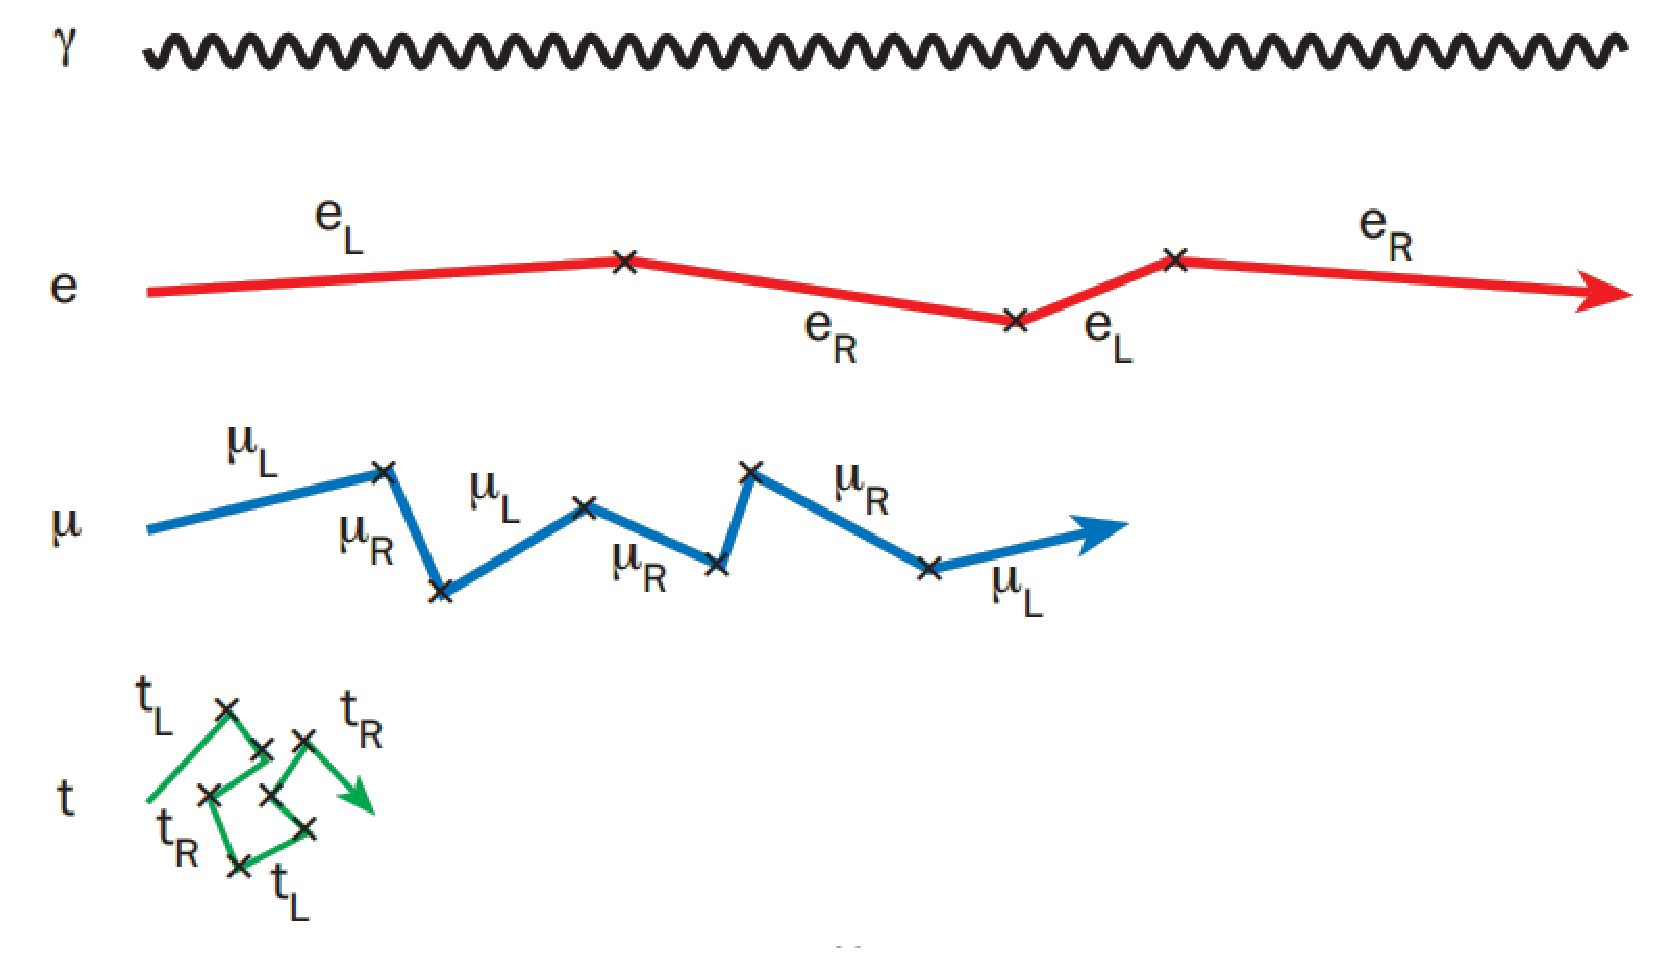
\includegraphics[width=0.4\textwidth]{figures/leptonMass.eps}
\caption{Leptons acquire mass by interacting with the Higgs field.  Figure taken from [CITE]}
\lable{fig:leptonMass}
\end{figure}
When neutrinos were thought to be massless, they were introduced into the Standard Model as spinor fields with no right-handed component.  The Higgs, which changes the chirality of the particle it interacts with, could not interact with the neutrino because it had no right-handed state to convert to.  The ansatz of a solely left-handed neutrino, then, created a massless neutrino in the Standard Model.  As experimental evidence has overwhelmingly favored a massive neutrino, it became necessary to modify the theoretical treatment of the neutrino.  One approach is to assume that the neutrino, like the SM leptons, is a Dirac fermion and has a left-handed component as well as a right-handed component, allowing the Higgs field to interact with the neutrino as it does for the leptons.  There is another approach to generate massive neutrinos that is not solely dependent on the Higgs field.  If neutrinos are Majorana fermions, that is, unlike Dirac fermions they are their own antiparticles, then the right-handed component of the neutrino field introduces an independent mass term.  When left-handed neutrinos interact with the background Higgs field, the heavy right-handed neutrino with mass $M$ can only exist for a short time without violating the Pauli principle.  It quickly interacts with the Higgs background, transforming back into a left-handed neutrino.  The mass scale of the neutrino is then $m/M$, where $m$ is the mass due to interaction with the Higgs field.  The advantage of the Majorana neutrino is that the scale of its interaction with the Higgs field can be comparable to that of other leptons; its small mass can be acheived by assuming a large $M$.  Majorana neutrinos also provide an explanation for baryon assymetry.  
\begin{figure}[htp]
\centering
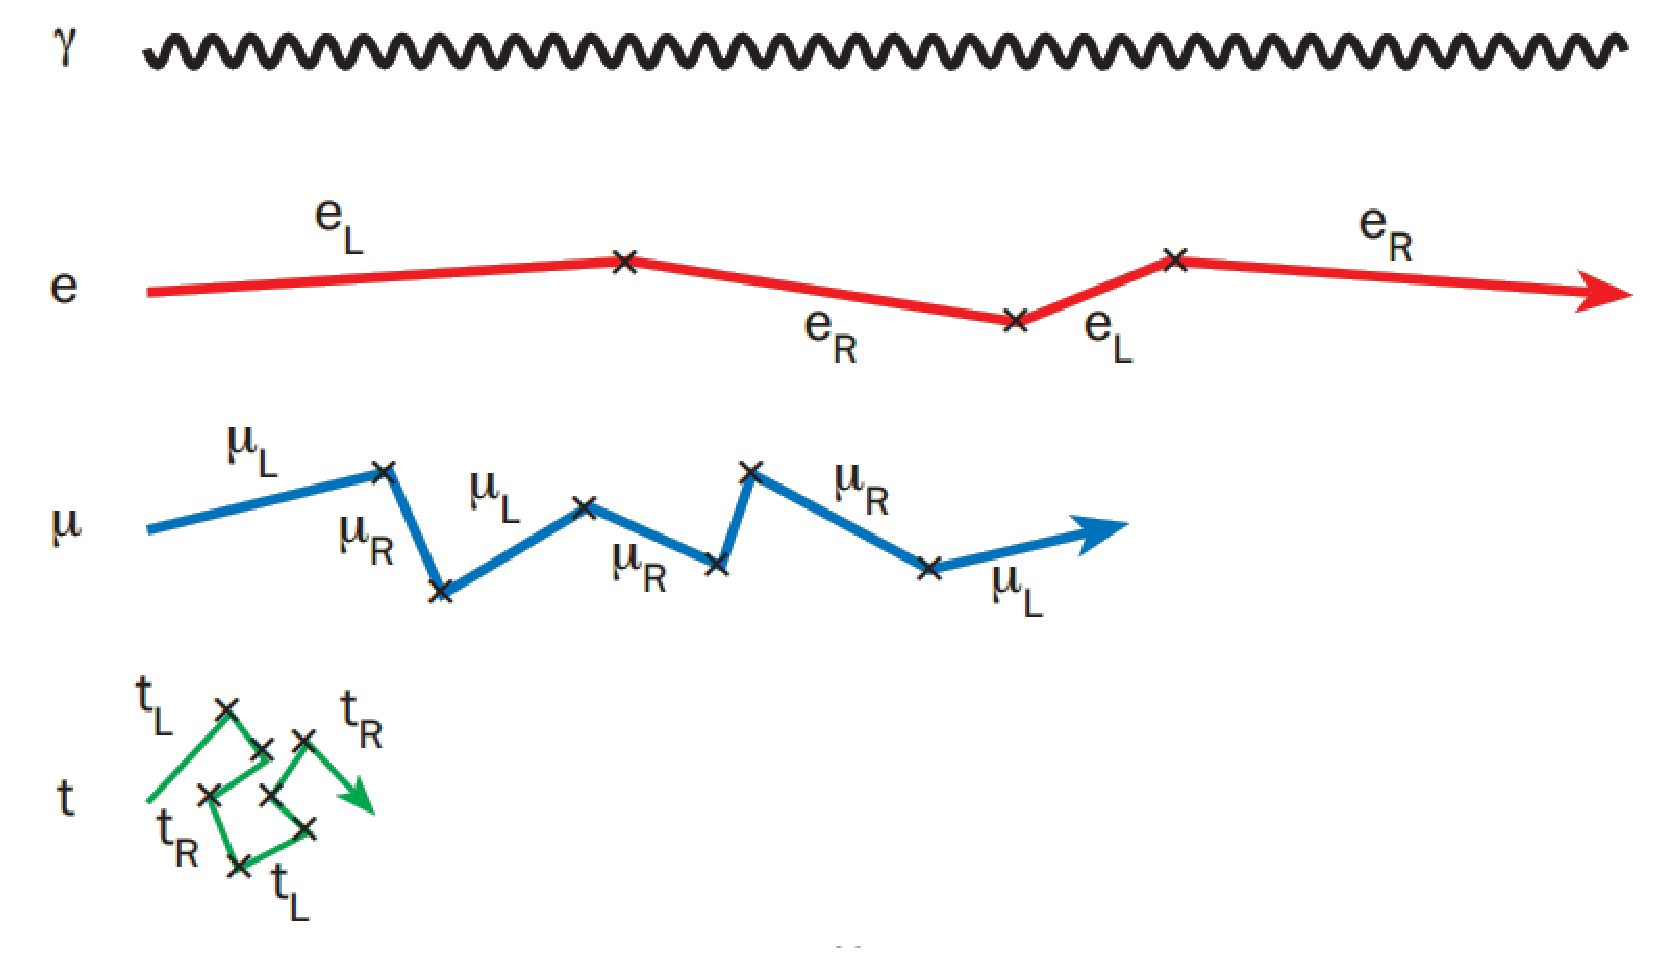
\includegraphics[width=0.4\textwidth]{figures/leptonMass.eps}
\caption{It is not known what type of particle the neutrino is; it is possible to introduce them into the Standard Model as either Dirac or Majorana fermions.  Figure taken from [CITE]}
\lable{fig:leptonMass}
\end{figure}  

Long-baseline experiments have determined that neutrinos are massive and have measured their mass differences and mixing angles to impressive accuracy, but much of their fundamental nature is still not understood.  That they could potentially play a significant role in many areas of physics provides significant motivation to build experiments that are sensitive to these neutrino ``parameters.'' One type of experiment that is sensitive to the Dirac or Majorana nature of the neutrino is a search for a process called neutrinoless double-beta decay (\zvbb).  Neutrino-full double-beta decay (\tvbb) is a process that has been observed in a number of nuclei and is the simultaneous beta-decay of two protons into two neutrons.  If the neutrino is a Majorana fermion, it would be possible for the neutrino to become an internal line.  This process would be impossible if the neutrino were not its own antiparticle; observation of \zvbb would confirm the Majorana nature of the neutrino. 
\begin{figure}[htp]
\centering
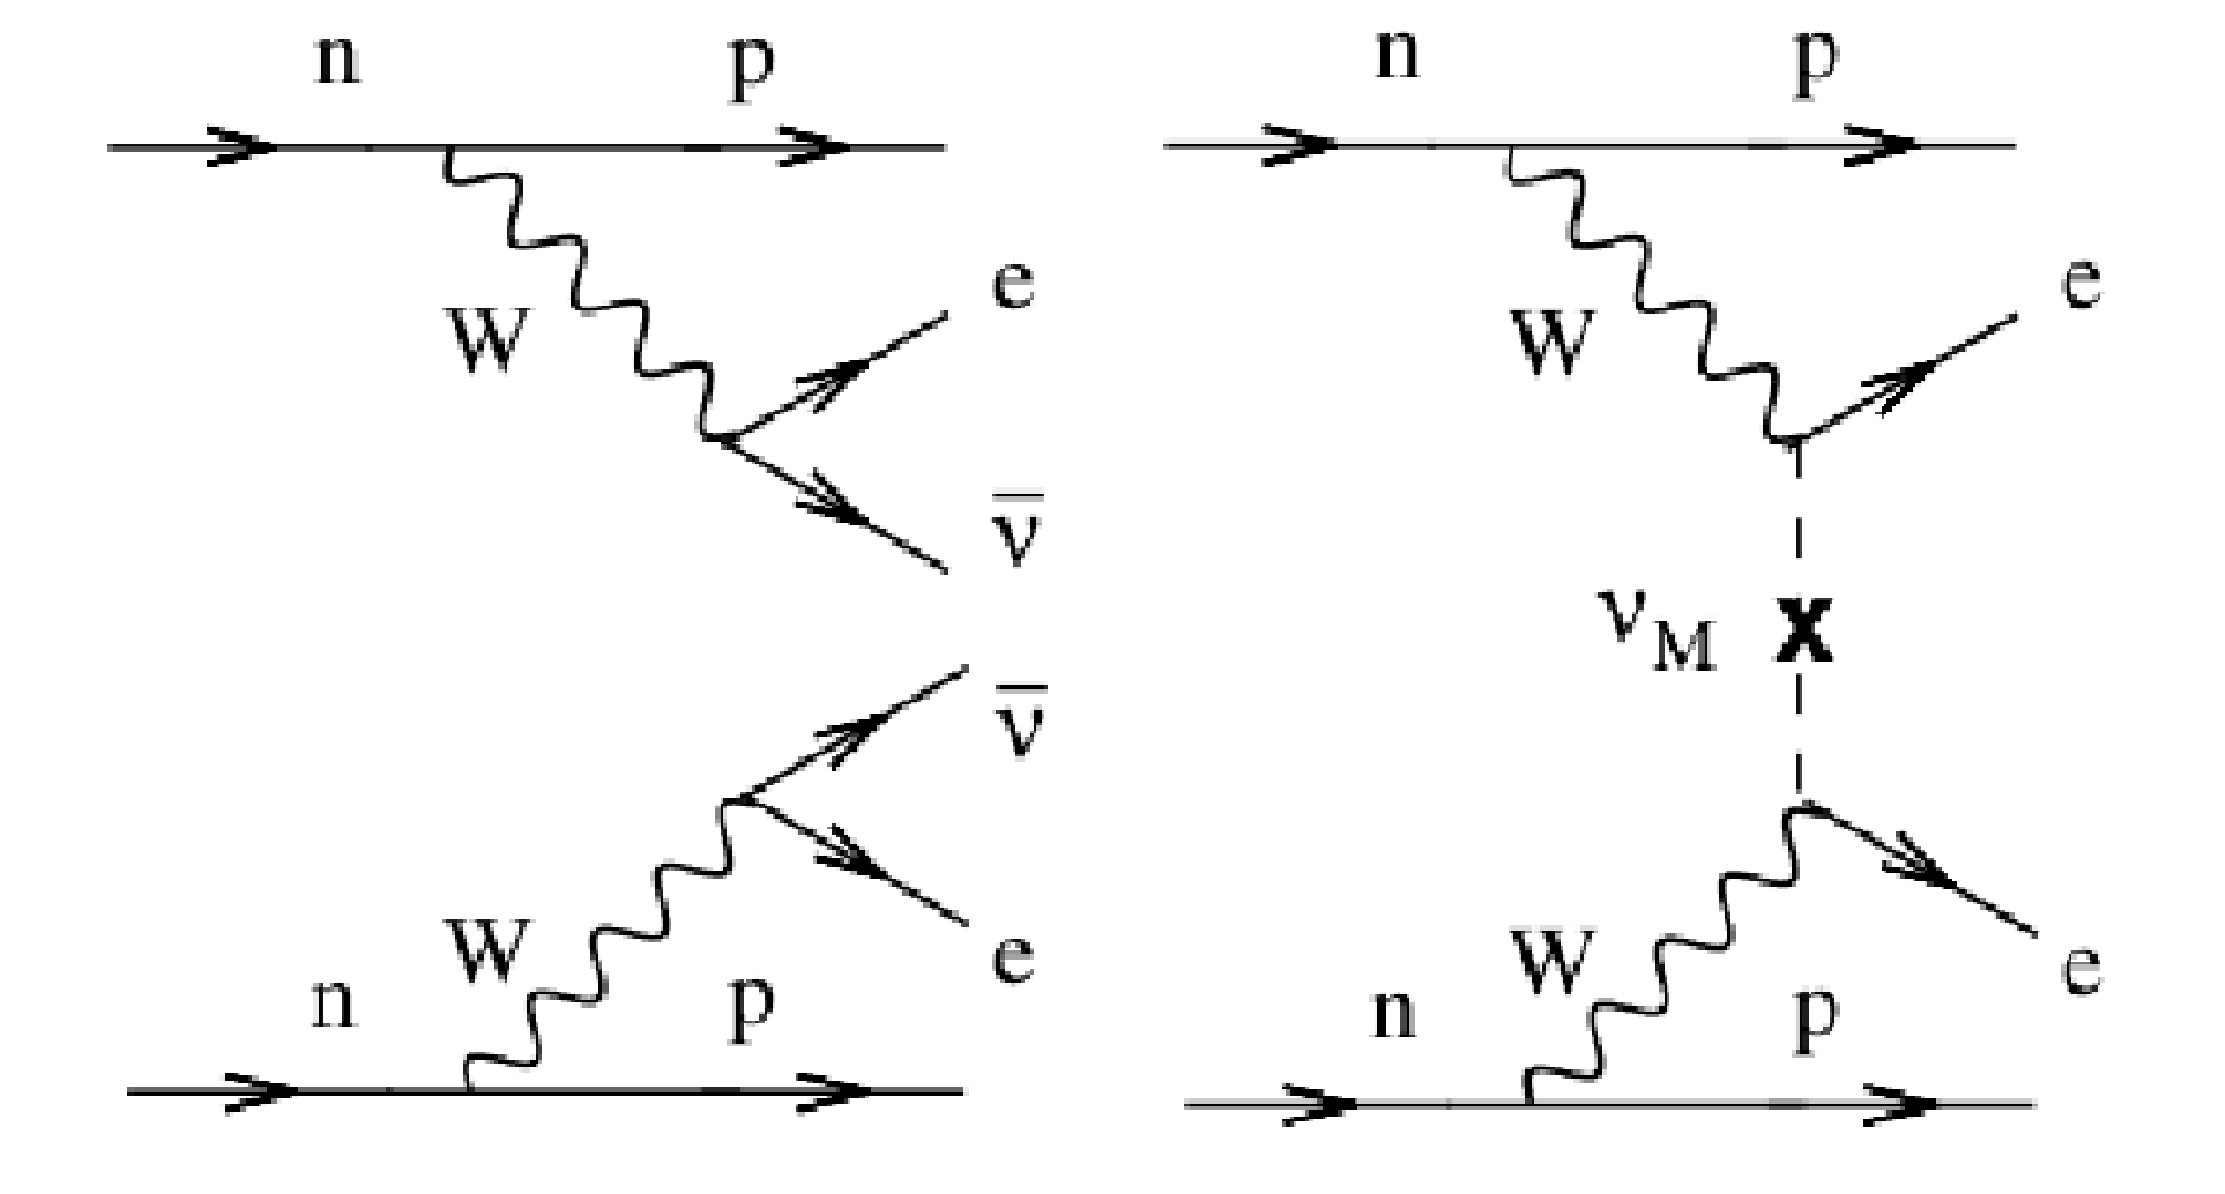
\includegraphics[width=0.4\textwidth]{figures/feynman2.eps}
\caption{Double beta decay.  Both the observed \tvbb and the hypothesized \zvbb modes are shown.  Figure taken from [CITE]}
\lable{fig:leptonMass}
\end{figure}
It should be noted that measured lifetimes for \tvbb are extremely long, on the order of $10^{\langle}m_{\beta\beta}{\rangle}^2{20}$~yr.  The expected lifetime for \zvbb, if it exists, will be even larger due to the supression of the right-handed component of the neutrino; the IGEX experiment [CITE] places the current limit at $>1.57\times 10^{25}$~yr.  This long lifetime makes \zvbb searches an impressive experimental challenge.  However, they are currently the only way to explore crucial properties of the neutrino.  Aspects of these experiments are discussed in the next section.

\section{\zvbb searches}
\begin{comment}
Discuss \zvbb process and sensitivity to nature of neutrino.
Discuss concurrent sensitivity to hadron part
I feel like I should discuss ongoing searches but not in much detail?  Relevant information is: expected lifetime, mass, expected counts/year, expected limits?
Okay, yes.  Here is how this section could go: discuss the process and the resulting equation for the lifetime, and then talk about each of the components of the equation.  START with the discussion of the lifetime - can include details of ongoing experiments there.
\end{comment}

Searches for \zvbb are of interest not only because an observation would conclusively demonstrate that neutrinos are Majorana, but also because an observed rate gives information on the absolute mass scale of the neutrino.  The lifetime of \zvbb, assuming it results from the exchange of light Majorana neutrinos, is 
\begin{equation}
(T^{0\nu}_{1/2})^{-1} = G_{0\nu}(Q_{\beta\beta},Z)|M^{0\nu}|^2 {\langle}m_{\beta\beta}{\rangle}^2,
\end{equation}
where $G_{0\nu}(Q_{\beta\beta},Z)$ is the phase space factor, $|M^{0\nu}| = |{\rangle}f|O|i{\langle}$ is the nuclear matrix element, and ${\langle}m_{\beta\beta}{\rangle} \equiv |\sum{k}m_k U_{ek}^2|$ is the effective Majorana mass.  The phase space factor can be readily calculated [CITE] and is typically on the order of $10^{-14}$~yr$^{-1}$.  The mass term is the effective mass of the electron neutrino and, unlike long-baseline experiments, is sensitive to the mass scale of the lightests neutrino particle.  This dependence is shown in {\fig}~\ref{fig:effectiveMajoranaMass} for the three possible heierarchy schemes.  
\begin{figure}[htp]
\centering
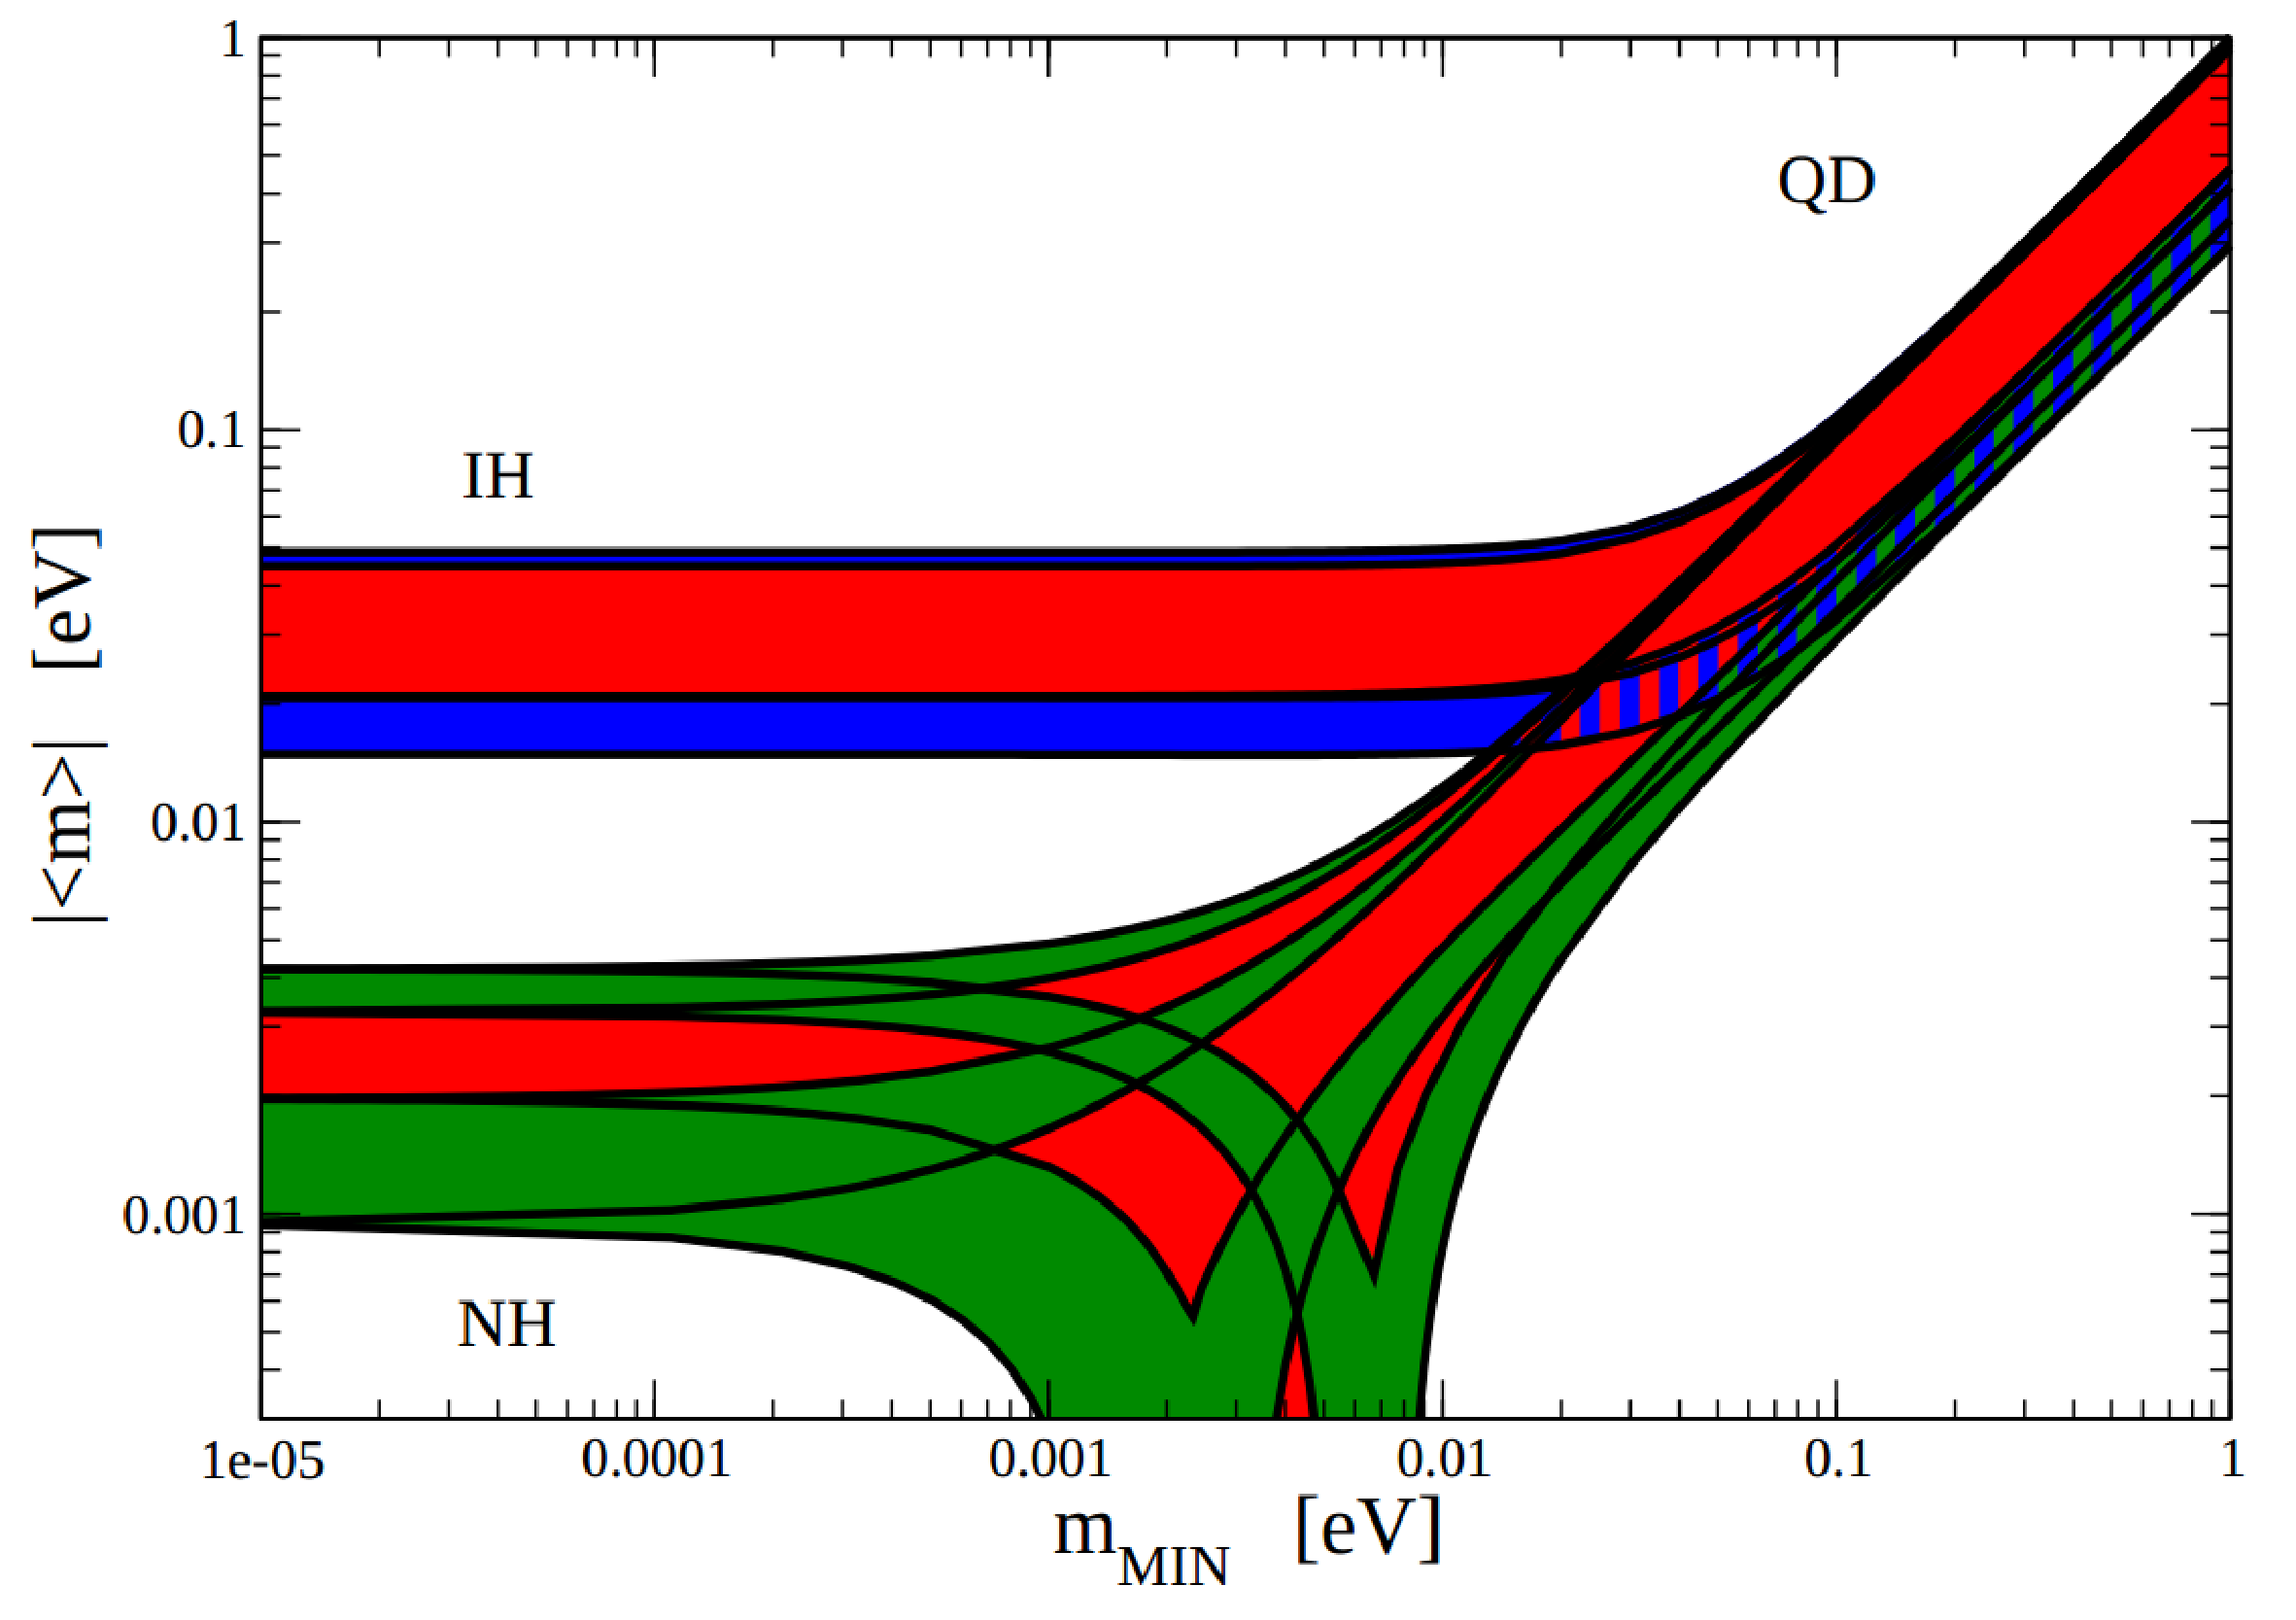
\includegraphics[width=0.8\textwidth]{figures/effectiveMajoranaMass.eps}
\caption{The effective Majorana mass in different heirarchy schemes.  Figure taken from \cite{PDG}.}
\lable{fig:effectiveMajoranaMass}
\end{figure}

The hadronic dependence of the lifetime, \NME, is sensitive to the initial and final nuclear wavefunctions.  Details of these calculations are discussed in {\chap}~\ref{chap:nucl}, but it should be noted that calculated \NME values for most candidate nuclei vary by as much as a factor of 5.
\begin{figure}[htp]
\centering
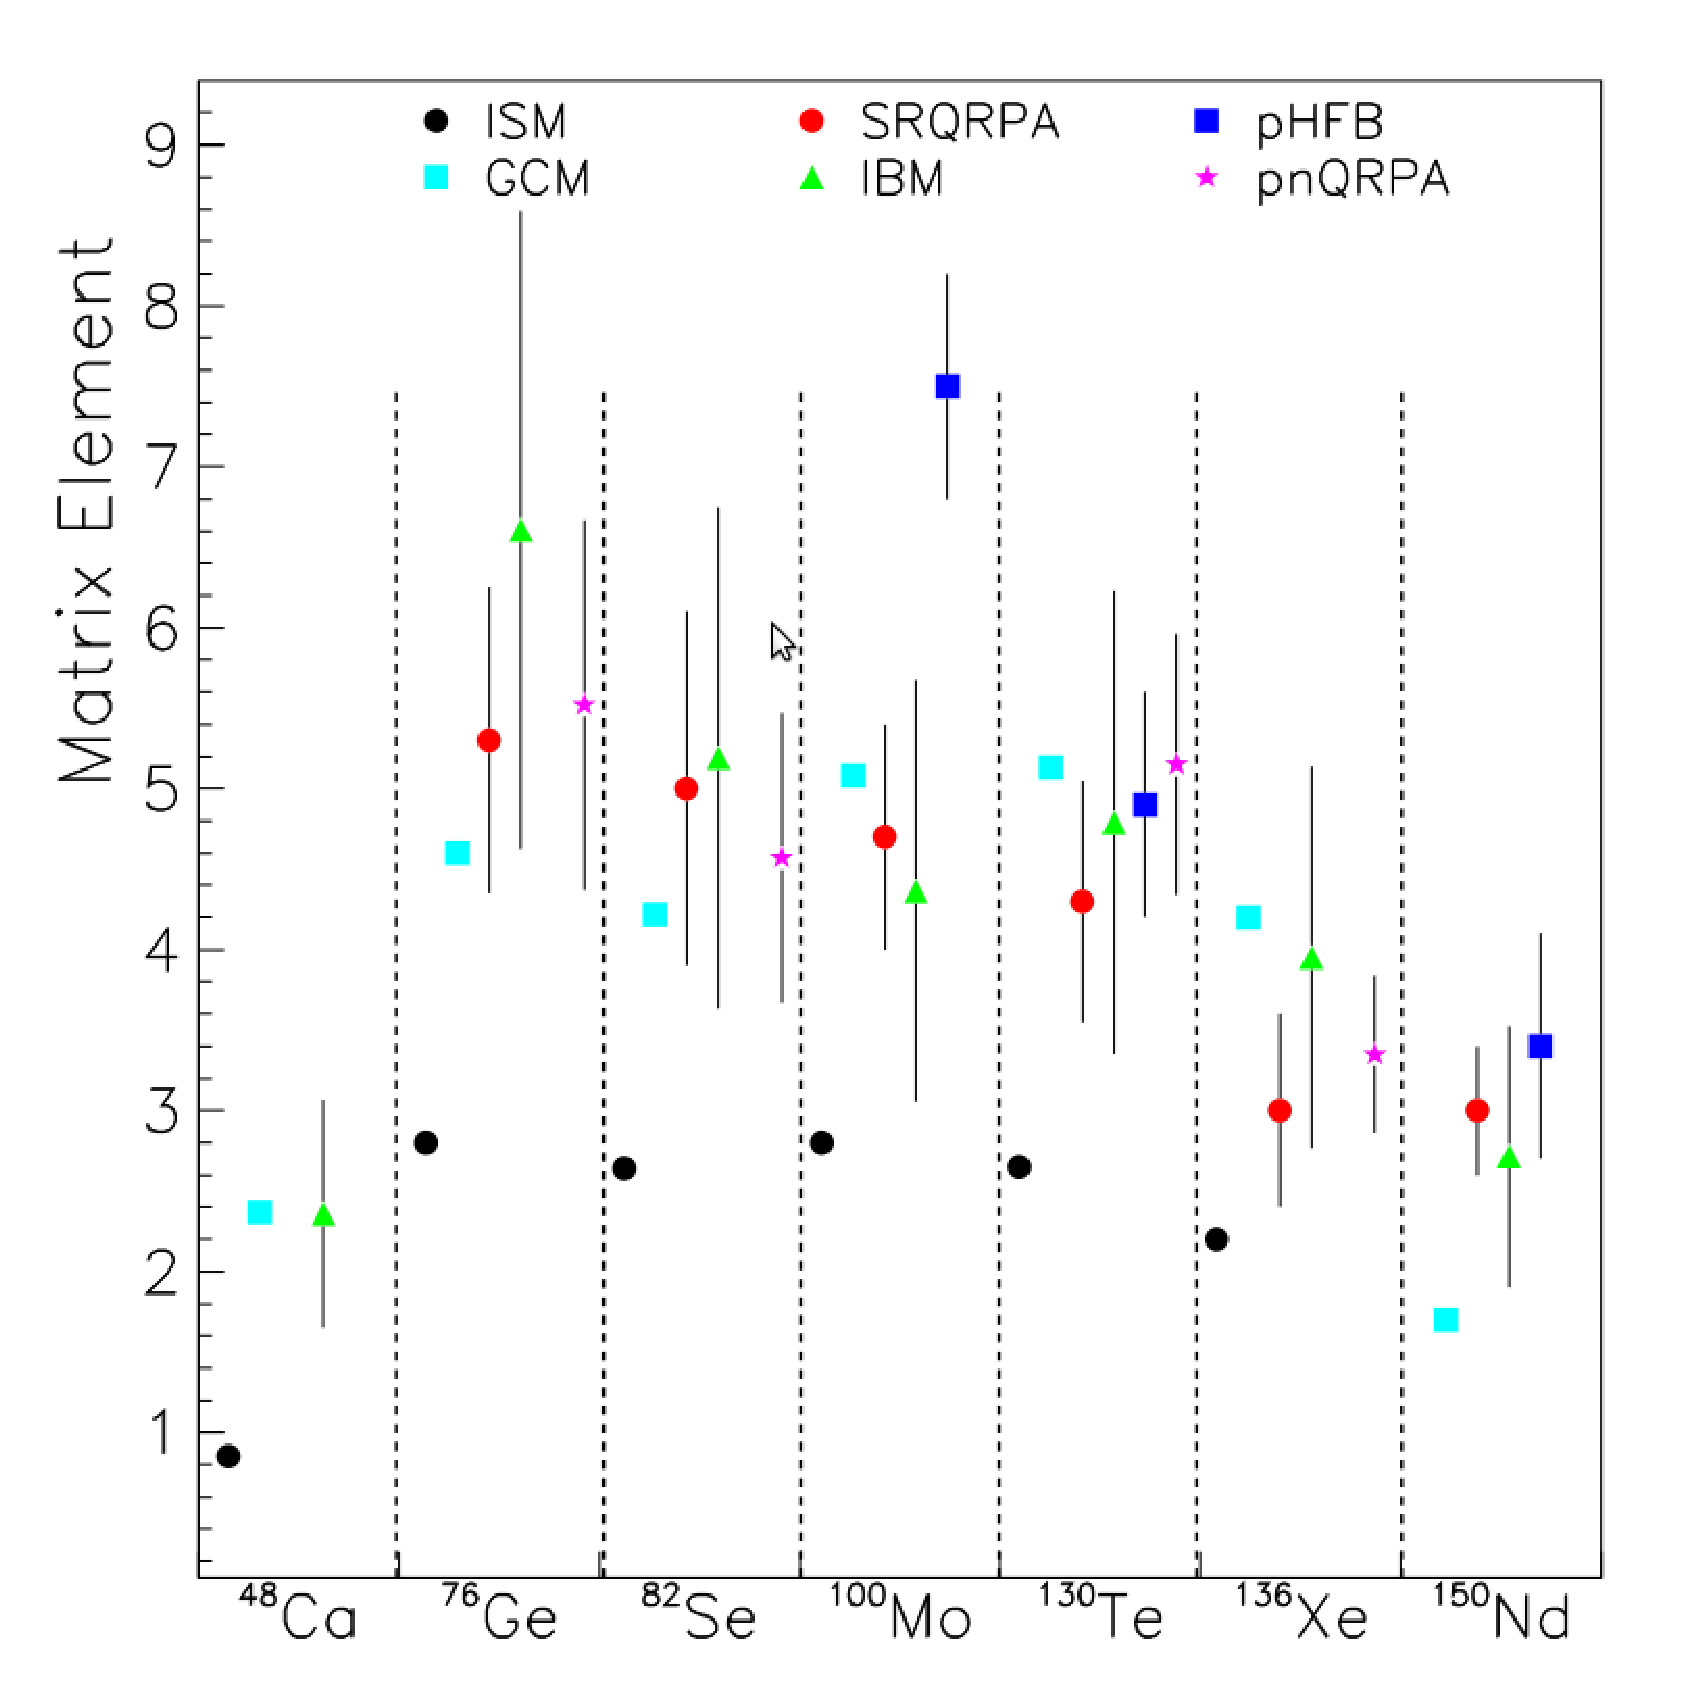
\includegraphics[width=0.8\textwidth]{figures/differentNME.eps}
\caption{Calculated \NME for candidate \zvbb nuclei.  The models used are the Interacting Shell Model (ISM), self-consistent renormalized quasi-particle random phase approximation (SRQRPA), proton-neutron quasi-particle random phase approximation (PNQRPA), generating coordinate method (GCM), and the interacting boson model (IBM).  Figure taken from \cite{zvbbReviewSchwingenheuer}.}
\lable{fig:differentNME}
\end{figure}  
This uncertainty in \NME directly affects the limits that can be placed on the neutrino mass scale if \zvbb is observed.  Transfer reactions, discussed in {\chap}~\ref{chap:nucl}, offer valuable experimental data that can be used to understand which models are most appropriate for these nuclei and improve the accuracy of the calculations.  The topic of this thesis is the two-proton transfer reaction, which is also discussed in {\chap}~\ref{chap:nucl}.

Nuclei that are suitable for \zvbb experiments are those that are stable against single beta decay but energetically allowed to double-beta decay.  This is the same group of nuclei in which \tvbb has been observed, and in fact the \tvbb process is a significant background to \zvbb.  The nuclei $^{48}$Ca, \Ge{76}, \Se{82}, $^{100}$Mo, $^{130}$Te, $^{136}$Xe, and $^{150}$Nd have been used to search for the process in past and present experiments.  Because of the uncertainties on \NME for these nuclei, it is not clear which, if any, would enjoy a shorter $T^{0\nu}_{1/2}$.  So many different experiments have arisen because each candidate nucleus offers different advantages in experimental design.  \Ge{76} is an appealing candidate because the active volume also serves as the detector, and Ge crystals are well understood.  Experiments using \Ge{76} are also important becuase the Klapdor-Kleingrothaus experiment, which claimed an observed \zvbb signal [CITE], used \Ge{76} crystals.  Other nuclei are appealing because they have high abundance.  This is the case for $^{136}$Xe, which is currently being used by the EXO-200 collaboration [CITE].  Experiments using $^{136}$Xe are typically time projection chambers (TPC), which are able to strongly reduce background by reconstructing the momenta of particles in a decay.  Using $^{136}$Xe is particularly appealing becuase large quantities are readily available, reducing the cost of increasing the mass scale of the experiment.  Another candidate nucleus, $^{130}$Te, is frequently used in experiments using bolometry to detect \zvbb.  A summary of \zvbb searches is shown in {\tab}~\ref{tab:experiments}.
\begin{table*}
\centering
\ra{1.3}
\begin{tabular}{@{}llllll@{}}\toprule
experiment & isotope & mass [kg] & method & start/end & ref. \\
\midrule
past experiments \\
Heidelberg-Moscow & \Ge{76} & 11 & ionization & -2003 & \cite{} \\
Cuorcino & $^{130}$Te & 11 & bolometer & -2008 & \cite{} \\
NEMO-3 & $^{100}$Mo, $^{82}$Se & 7,1 & track + calorim. & -2011 & \cite{} \\
\vspace{0.1cm}

current experiments \\
EXO-200 & $^{136}$Xe & 175 & liquid TPC & 2011- & \cite{} \\
Kamland-Zen & $^{136}$Xe & 330 & liquid scint. & 2011- & \cite{} \\
GERDA-I/GERDA-II & \Ge{76} & 15/35 & ionization & 2011-/2013- & \cite{} \\
CANDLES & $^{48}$Ca & 0.35 & scint. crystal & 2011- & \cite{} \\
\vspace{0.1cm}

funded experiments \\
NEXT & $^{136}$Xe & 100 & gas TPC & 2015 & \cite{} \\
Cuore0/Cuore & $^{130}$Te & 10/200 & bolometer & 2012-/2015- & \cite{} \\
Majorana Demo & \Ge{76} & 30 & ionization & 2013 & \cite{} \\
SuperNEMO Demo/Total & \Se{82} & 7/100 & track + calorim. & 2014-/?? & \cite{} \\
SNO+ & $^{150}$Nd & 44 & liquid scint. & 2013 & \cite{} \\
\bottomrule
\end{tabular}
\caption{\zvbb experiments.  From \cite{}.}
\label{tab:experiments}
\end{table*}

Searches for \zvbb offer access to unique areas of neutrino physics.  Confirmation of the process would demonstrate that neutrinos are Majorana in nature and would also provide a measurement of the absolute mass scale of the electron neutrino.  The dependence of the lifetime on \NME poses a difficulty because the current uncertainty in calculations limits the sensitivity to the neutrino mass scale and also increases the difficulty of planning experiments that search for the process.  Nuclear transfer experiments provide information that can help reduce the uncertainty of \NME calculations, and this thesis focuses on two-proton transfers onto the Ge system.  The impact of such a transfer experiment is discussed in {\chap}~\ref{chap:nucl}.


% % uncomment the following lines,
% if using chapter-wise bibliography
%
% \bibliographystyle{ndnatbib}
% \bibliography{example}
